%===================================== CHAP 3 =================================

%\chapter{Method}
\chapter{Conceptual design}
%\chapter{Approach and methodology}

\section{Overall Approach}

%%forklare hva jeg prøver å gjøre på en generell måte. introdusere pipelinen
Wikipedia is a web page presenting articles for the user. This leads to high focus on the usability related to users searching and reading articles. Because of this one can say that their articles are stored as an atomic entity in their database. An article has no internal structure, except for the markup used to present it. That means that a process is needed to identify and extract examples from Wikipedia articles. This 
project %%Hva burde jeg kalle dette?
looks into the pipeline technique for this process. As explained in section \ref{pipeline}, a pipeline consist of multiple independent processes loosely coupled.\\


%\section{Prerequisite knowledge}

\section{Pipeline} \label{cd_pipeline}

%%Write something about the approach being for data mining. Where to different methods where explored. Focus on how it was done.
\subsection{Creating the pipeline} \label{custom-pipeline}

%%del opp deler av pipelinenen i subsectioen under denne sectionenen, del opp i SQL og elastic search. Ta med prosessen som fører til det

\begin{figure}[h]
\caption{A conceptual overview of the pipeline used to extract and index examples}
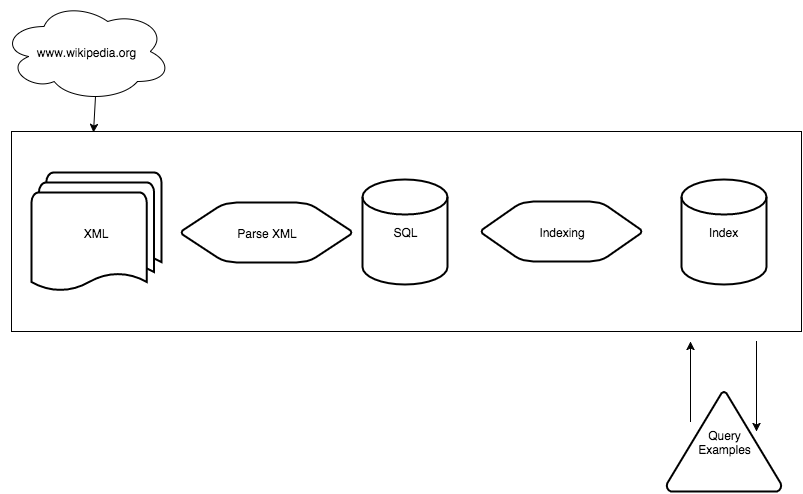
\includegraphics[width=\textwidth]{PipelineConcept}
\end{figure}



Based on what was discussed in section \ref{smila}, it was decided to not use the SMILA system and its utilities itself, but instead look at how SMILA approaches the problem and take inspiration from that. Therefor other methods were considered, which mainly consisted of building the pipeline from scratch. Tailoring the different sub-processes for this project and organizing them in a pipeline, was decided to be the best course of action. The first issue to be settled regarded the format of the source data. SMILA fetches information by crawling the web, in our case Wikipedia\footnote{www.wikipedia.org}, but using a web-crawler is a very general method. Since this project were only going to use Wikipedia, the extraction method could be more specific. An XML-dump from a snapshot of Wikipedias database fits perfectly in terms of simplicity and stability for this project. This dump contains all the articles of Wikipedia in their newest version.

%%better transitioning between these two sections

All the sub-processes in the pipeline are loosely coupled. This means that they are fully independent given the correct input. This also allows the pipeline to easily swap out sub-processes without affecting the rest of the system. The SMILA pipeline also delivered a high degree of parallelity. This is a property the current version of the pipeline created from scratch does not have. This is because functionality was prioritized above efficiency during development. 

\subsection{Extracting data from XML-dump to SQL}

The source data used for input to the pipeline uses the XML format. On the top level of the XML douments there exists article elements marked with an article tag. Each article element represents a page on Wikipedia and thus contains metadata about the page as well as the content itself. All this data forms a XML document with a size of 50GB.
A parsing process was created in JavaScript running locally on a node.js server to handle a document of that size. This process reads the XML-document as a stream, buffering line by line, and then identifies article elements and saves the relevant data from it to an object in memory. Then for each article, the process looks at the sections and selects the ones that contains an example. It then parses that article into a JavaScript object with the relevant data. As it iterates over the articles, the process stores the data in a relational database. The database stores data about whole articles, specific sections and references in the sections. Relations between these are also stored, and are used in the next step of the pipeline, when this data will be used to form example entities. 

\subsection{Building an index of examples from SQL}
%write about elastic search
The first step in building the index is fetching data from the database to form examples. Virtual tables called \textit{views}%%referanse her
, are used in the database to normalize%%referanse her
 the data on a format which the index will be using.

Elasticsearch was chosen as the tool for building the index. Section \ref{elasticsearch} explains why it is a good choice for this project. A simple Java process fetches the views from the database and creates objects based on models representing examples. References to other examples and which categories the examples are also added here. The example model has a one-to-one relationship to the examples represented in the Elasticsearch index, so the objects are directly converted to JSON and inserted into the index. To configure and query the index, Elasticsearch servers a HTTP API. This API is used before building of the index to specify behaviour of different fields, and after for searching the complete index.


\section{Querying examples}

\begin{figure}[h]
\caption{A simple overview of the users interaction with the examples}
\includegraphics[width=\textwidth]{UserInteraction}
\end{figure}

\subsection{General idea}
When the source data, consisting of wikipedia pages, has been processed through the pipeline described in section \ref{cd_pipeline}, the final result is an index built up of examples. Having just an index is not very useful without an easy way of interacting with it though. Therefor a user friendly, web based search interface has been created. 

The interfaces main objective is to assist the user in finding relevant examples and to present these examples to the user in a helpful manner. To present the examples, the interface use HTML and CSS from the live version of Wikipedia from its web server. To find relevant examples, the interface helps the user in two ways. The first one is simply using keywords entered in a search field by the user. The second way is when the user has already selected an example he finds relevant, the search interface will then use this example to find similar examples.

\subsection{Querying by keywords}

The users first interaction with the interface is by using the search field. In this field the user will type in keywords which will be used in a query sent to Elasticsearch. Elasticsearch will then use the tf-idf algorithm to match the search phrase to fields contained in the example. The fields that will be used for the matching are introduction, content, title and categories. By boosting the importance of some fields, the query is fine tuned to deliver a relevant collection of examples based on the keywords in the search phrase.


\subsection{Querying by examples}
The collection of examples returned by the users first query is presented in a list. This list allows the user to browse through the returned examples and select an example. When this example is selected a new query is automatically performed to Elasticsearch. This query is based on the selected example and is an \textit{compound query}, which means it is a query that wraps around sub queries. One of those sub queries used by this query is a filter. This sub query filters results based on common categories. It also filters on section id, to exclude the same example. The second part of the query is another sub query that performs a match between references and page titles. This match uses an analyzer to make the query act like a \textit{full text search}. %ta med referanse her
By combining these sub queries the interface presents two lists of related examples to the user, one based on references into the current example, and a second one based on references from the current example. 

\section{Analysis of examples} \label{examples-section} %% må skrives om til hvordan vi faktisk drar nytte av det, når det blir implementert
%strucutre/characteristics of an example\\
%what is good and bad example

\subsection{An example}

An example is used as a tool to better understand a topic. It is usually used together with an explanatory text, where the example is a minor part of it. Examples are rarely presented standalone since they often required a certain degree of context. If this context is fused into the example, it often tends to make the example very complex and too troublesome to use efficiently. Because of this, an example can often be looked at as an appendix to a text regarding a subject. 


%%Finn et annet ord for persons?
Persons who want to learn about a certain topic, but already knows the basic context may prefer to skip the explanatory text and only look at the examples. This projects tries to exploit the fact that examples acts as an appendix to a subject and index them based on that. This attempts to give persons, trying to expand their knowledge within a topic, a more preferable way of doing so.

\subsection{Comparing examples} \label{comparing_examples}

To find common properties of examples is very difficult. Nearly impossible if you compare across different domains. When comparing two examples within the same domain and topic, there will still be different approaches and techniques of explaining, which still makes it hard to directly compare them. As a consequence of this, a highly qualitative and subjective analysis has been made for examples within the Game Theory domain. 

Different key properties have been identified and examined across different topics. Some properties are connected to the structure and presentation of the example, while others are based on the contents. From examining topics within Game Theory, a list of properties of an example were designed. Table \ref{table:1} displays these properties with a brief explanation.

\begin{table}[h!]
\centering
\begin{tabular} {|| p{5em} | p{23em} ||} 
 \hline
 Name & Description \\ [0.5ex] 
 \hline\hline
 Figures & Graphics and drawings contained in the example. \\ 
 Length & The length of the example, can be both words and characters. \\
 Domain & Which domain the example belongs to. \\
 Source code & If source code is used for explaining principles. \\
 Equations & If equations is used to explain the example \\
 Analogies & When an real world example is used to explain a theoretical one. \\
 Sub sections & An example that is divided up in smaller parts or sections that offer different angles of explanations for the example. \\
 Walkthrough & A step by step guide that solves a problem. \\
 Iterations & Several iterations that gradually increase the complexity of the explanation \\
 References & How often the example refers to figures or other examples and articles \\ [1ex] 
 \hline
\end{tabular}
\caption{Properties of an example and a description of them.}
\label{table:1}
\end{table}


\subsection{Structure of a good example} \label{good_example}

The structure of an example is mostly defined by how it utilizes the properties mentioned in table \ref{table:1}. It is important to establish that whether the example uses a property or not, is an all to easy approach. The combination of the values these properties contains is significant, especially the property describing the domain. This has lead to a narrow approach domain-wise when looking into different examples.
When trying to identify the structure of a good example, there have been selected a few topics within the Game Theory domain. Then for a certain topic, two or three examples have been compared to each other.  

For the topic \textit{Pareto efficiency} the first example examined is\\ https://www.economics.utoronto.ca/osborne/2x3/tutorial/PEDEX.HTM. This example builds up its explanation step by step with several iterations. Each iteration is a bit more complex than the previous. This enables the example to cover the topic with a certain depth. The second example is https://www.tau.ac.il/~spiegel/teaching/inter-micro/Crueso.pdf. This example is very long and detailed. In addition to a large amount of text, it also uses equations to a substantial degree. Initially the first example feels better, it is definitely easier to grasp the concept of \textit{Pareto efficiency}. The second example focuses more on the mathematical part, and there will most likely exist some persons who prefer this. 

\subsection{Using the results}

As explained in section \ref{good_example}, the properties of a good example may change based on the person making use of it. For the index built in this project it is important to acknowledge this. By using the properties listed in table \ref{table:1} and the structure of good examples, a smarter search can be formed. When the user is browsing through examples, the list of related examples can then be arranged in fashion that is for instance based on difficulty of the example. This can give the user a natural feeling of progress when learning about a subject.

By using knowledge from section \ref{examples-sections} and input from the user, our search interface can compile two lists of related examples. These are the lists will be presented to the user, to make him able to explore further examples. 



\cleardoublepage